\documentclass[10pt,letterpaper]{article}
\usepackage{tools}
\usepackage{enumitem}
%\settextfont{B Nazanin}
\usepackage{lipsum}
\setlength{\parskip}{3mm}
\setlength{\parindent}{0mm}
\newcommand{\wid}{0.49\textwidth}
\newcommand{\widone}{60mm}
\begin{document}
\Large
\begin{center}
In the name of beauty

4th problem set solution of ComNet course
\hl
\end{center}
Q1)
\begin{enumerate}[label=\alph*-]
\item
False. UDP provides more control to the sender side, with which e.g. the sender can start transmission at any time or rate it pleases. Under TCP however, constraints such as congestion control would show up.
%\item
%An application could have reliable data transfer while using UDP protocol.
\item
False. The length field in each UDP segment specifies the number of bytes in the UDP segment.
%\item
%If two UDP or TCP segments have different source IP addresses and/or source port numbers, but have the same destination IP address and destination port number, then the two segments will be directed to the same destination process via the same destination socket.
\item
False. Using less transmission rate in an end-to-end transmission, will increase sender utilization and decrease effective throughput (more on this later in question 4).
\item
False. The sender will retransmit that most recent packet it already sent.
\end{enumerate}

Q2)
\begin{enumerate}[label=\alph*-]
\item
$$
01110100
$$
\item
The complement of the event that the receiver detects an error, is the case where either no error really happened or the error was in declared in case of occurrence. The probability to the former one is $(1-p)^{32}$ and the latter one occurs when at least one bit column imposes silent-error with a probability of $q$. It is easy to show that
$$
q=\binom{4}{2}p^2(1-p)^2+\binom{4}{4}p^4
$$
and the probability of silent error becomes $1-(1-q)^8$. Hence we have
$$
p_{e-d}=1-[(1-p)^{32}+1-(1-q)^8]
$$
The error is detected in the message if at least one of the 8 bits of the checksum does not match along the corresponding bit column in the received segment. The complement of this event is when the receiver detects nothing abnormal and proceeds to deliver the packet to the Application layer. Such an either no-error or \textit{silent-error} must occur at each bit value, with a total probability of
$$
\left[
\binom{4}{0}p^0(1-p)^4+
\binom{4}{2}p^2(1-p)^2+
\binom{4}{4}p^4(1-p)^0\right]^8
$$
leading to the probability of error detection as
$$
P_{e-d}=1-\left[
1-
\binom{4}{1}p^1(1-p)^3-
\binom{4}{3}p^3(1-p)^1\right]^8
$$
\item
Similarly
$$
P_{s-e}=1-\left[
1-
\binom{4}{2}p^2(1-p)^2-
\binom{4}{4}p^4(1-p)^0\right]^8
$$
hence
$$
P_{e-d}\approx0.27\quad,\quad P_{s-e}\approx0.005
$$
\end{enumerate}

Q3)

%Assume a sender uses rdt 3.0 (stop-and-wait) protocol to send packets to a receiver. Consider three senarios as described in Figure \ref{fig.1} where:
\begin{enumerate}[label=\alph*-]
\item
The sender will retransmit \texttt{pkt1} due to alerted TIMEOUT and will reset the timer. The procedure is kept on until the sender notices the correct reception of the packet. The receiver acknowledges the sender's successfully-arrived packet, which is pinged back to the sender and command it to head over for the next packet due to the FSM.
\item
Same as in part (a).
\item
This scenario leads to duplicate ACKs since the sender receives two ACKs for a same packet, the second one being received because of the second of transmitting the packet to the receiver. The receiver has really nothing to do more complicated; it will simply do the boring job of including the sequence number of the received packet in each ACK response!
\end{enumerate}
%\begin{figure}[ht]
%\centering
%%%%%%%%%%%%%%%%%
%\begin{subfigure}{\wid}
%\centering
%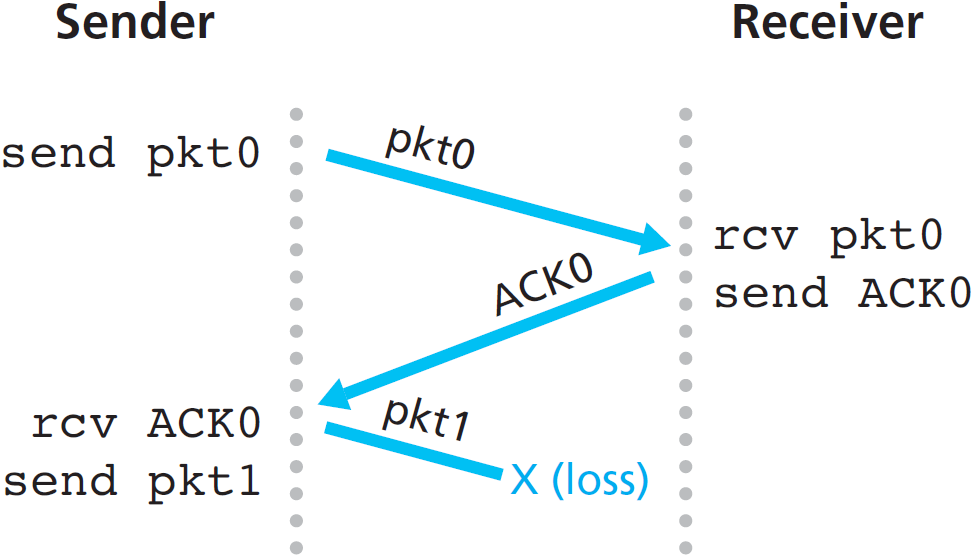
\includegraphics[width=\widone]{rdt1}
%\caption{Packet Loss}
%\end{subfigure}
%%%%%%%%%%%%%%%%%
%\begin{subfigure}{\wid}
%\centering
%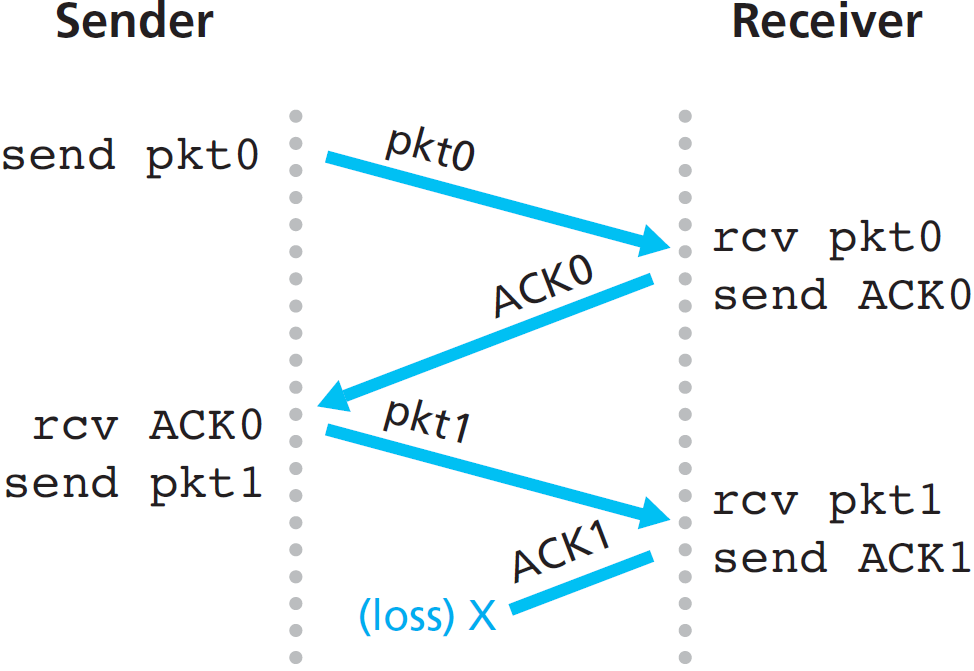
\includegraphics[width=\widone]{rdt2}
%\caption{ACK Loss}
%\end{subfigure}
%%%%%%%%%%%%%%%%%
%\begin{subfigure}{\wid}
%\centering
%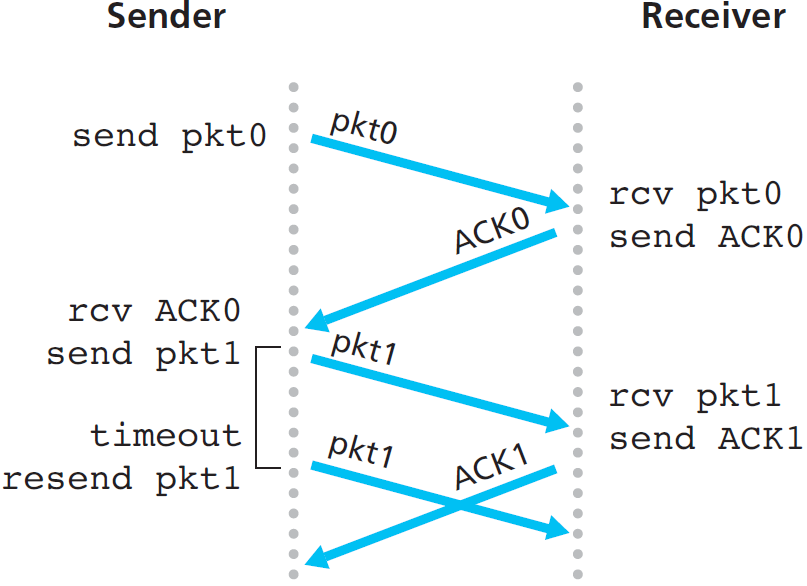
\includegraphics[width=\widone]{rdt3}
%\caption{Improper TIMEOUT}
%\end{subfigure}
%%%%%%%%%%%%%%%%%
%\caption{Three possible scenarios for rdt3.0 sender}
%\label{fig.1}
%\end{figure}

Q4)

%Consider rdt 3.0 protocol in an ideal case, that is, with no bit error or loss. The sender transmits $n$ packets consecutively using pipelining. Assume $L=500$ bytes is the packet size, $R=4\text{Gbps}$ is the transmission rate, the distance between sender and receiver is 1000 km and the propagation speed is $2\times 10^8$ m/s. Suppose the ACK messages will not suffer transmission time due to small packet size.

\begin{enumerate}[label=\alph*-]
\item
The sender would transmit $n$ packets in $n$ $\mu$sec with a RTT of 10msec. The sender utilization becomes
$$
U={{nL\over R}\over {nL\over R}+\text{RTT}}={n\over n+10000}
$$
\item
$$
U(n=1)\approx 0.0001
$$
Exploiting a link with lower transmission rate will help zero since it reduces the effective throughput (even though it improves the utilization a bit!).
\item
$$
U(n=8)\approx0.0008
$$
\end{enumerate}
%\newpage
%$$
%{nL/R\over nL/R+0.01}={nL\over nL+0.01\times R}R
%$$
%
%$$
%{nL\over }
%$$
%\newpage

Q5)

%Consider the Finite State Machine of protocol rdt2.1 as shown in Figures 2 and 3. Since the protocol of rdt2.1 generally works well with a channel with no packet loss, add a TIMEOUT to both the sender side and receiver side of rdt2.1 so as to avoid the infinity loop of waiting for lost packets (draw the modified FSM for both the sender side and receiver side).
\begin{figure}[ht]
\centering
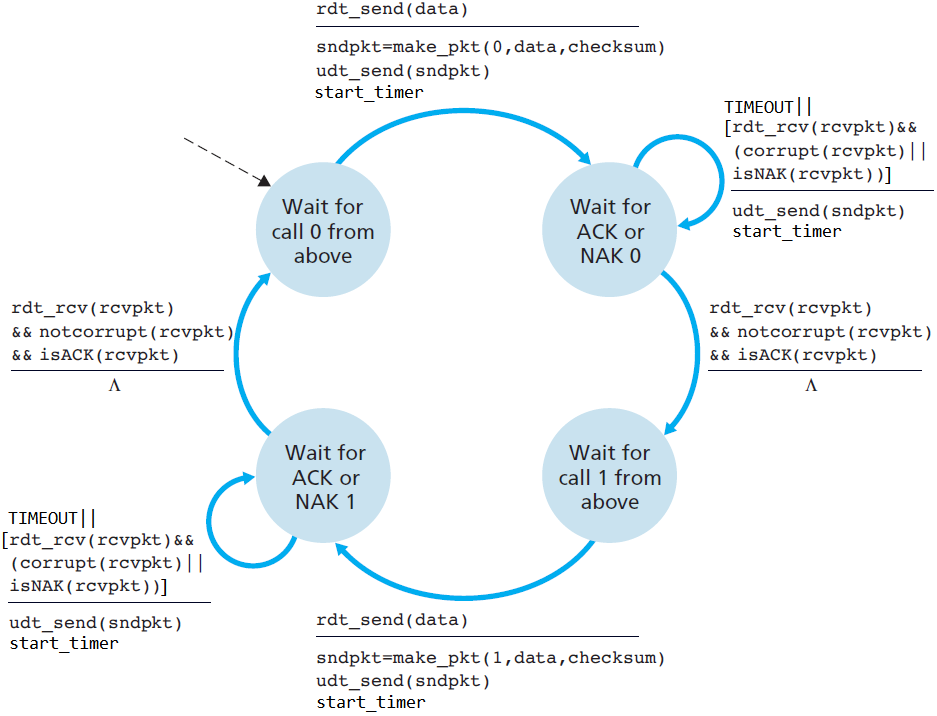
\includegraphics[width=150mm]{rdtsender_m}
%\caption{rdt2.1 sender}
\end{figure}
%\begin{figure}[ht]
%\centering
%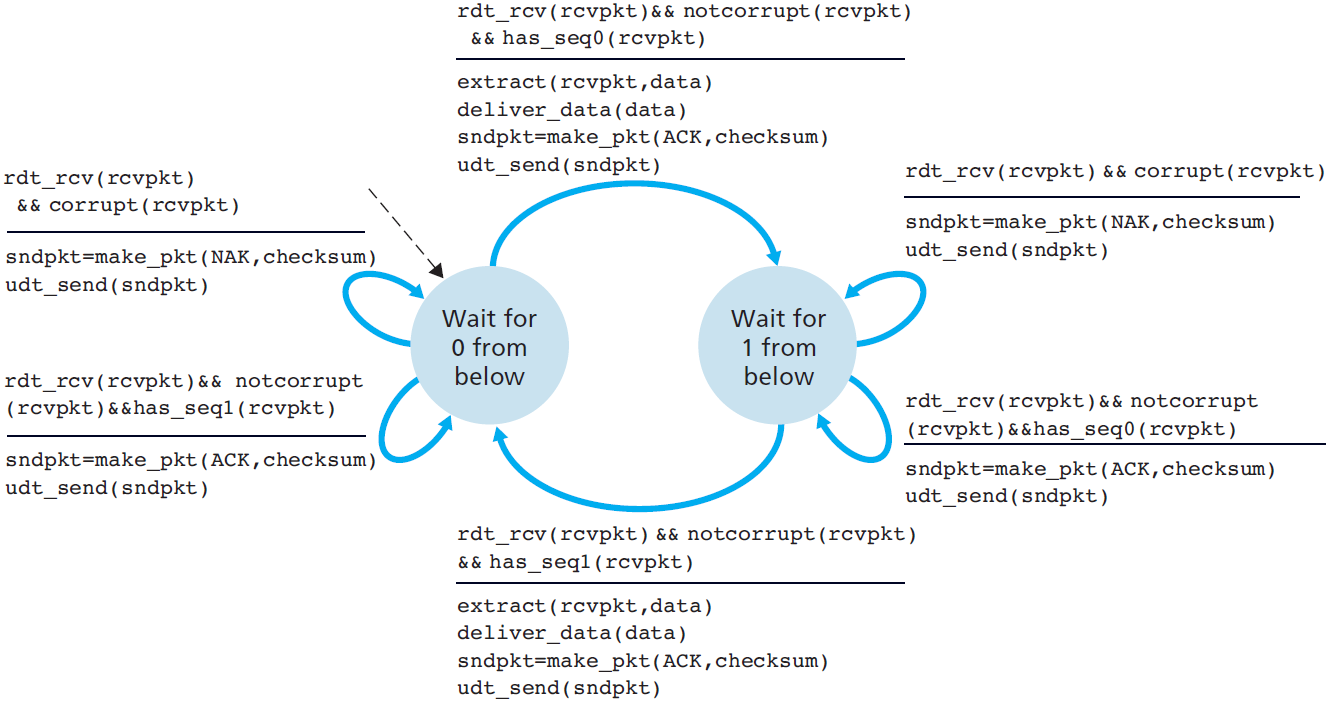
\includegraphics[width=150mm]{rdtrecv}
%\caption{rdt2.1 receiver}
%\end{figure}
%Determine the following statements as true or false with enough reasons.
%\begin{enumerate}[label=\alph*-]
%\item
%Both trasport and network layer protocols provide logical communication between processes running at different hosts rather than hosts themselves.
%\item
%Transport layer packets are refered to as \textbf{datagrams}.
%\item
%TCP ensures that the transmitted packets would finally reach their destination, however it makes no guarantee on the order of packets.
%\item
%The IP service model is a best-effort delivery service since it guarantees to deliver segments between communicating hosts, whether orderless or not.
%%\item
%%Cookies are used to keep track of user IDs in a stateless HTTP server.
%%\item
%%Link-layer switches are typically capable of processing the packets up to the layer 3.
%%\item
%%SMTP and FTP are examples of layer 1 protocols while TCP is a transport layer protocol.
%%\item
%%API is a set of rules 
%%\item
%%For economical reasons, exploiting optical fibers is not recommended in long-haul network
%\end{enumerate}
%
%Q2)
%\begin{enumerate}[label=\alph*-]
%\item
%Why is IP said to be an unreliable service and if so, how would TCP provide reliable data transfer on top of IP?
%\item
%Why are source and destination host port numbers included in segment headers? What problem could arise if they are ignored?
%\end{enumerate}
%
%Q3) Suppose Client A initiates a Telnet session with Server S. At about the same
%time, Client B also initiates a Telnet session with Server S. Provide possible
%source and destination port numbers for
%\begin{enumerate}[label=\alph*-]
%\item
%The segments sent from A to S.
%\item
%The segments sent from B to S.
%\item
%The segments sent from S to A.
%\item
%The segments sent from S to B.
%\item
%If A and B are different hosts, is it possible that the source port number in
%the segments from A to S is the same as that from B to S?
%\item
%How about if they are the same host?
%\end{enumerate}
%(Choose the port numbers at source and destination arbitrarily.)
%
%Q4) Consider the following Figure. What are the source and destination port values in the segments
%flowing from the server back to the clients’ processes? What are the IP
%addresses in the network-layer datagrams carrying the transport-layer segments?
%\begin{figure}[ht]
%\centering
%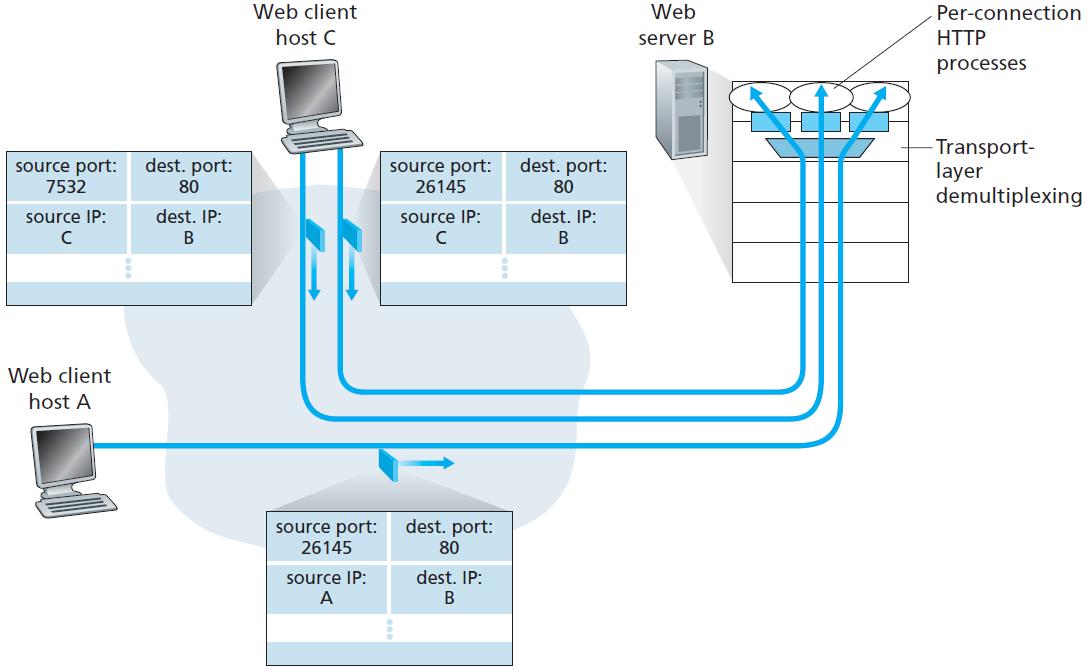
\includegraphics[width=180mm]{simnet}
%\end{figure}
\end{document}